%%%%%%%%%%%%%%%%%%%%%%%%%%%%%%%%%%%%%%%%%%%%%%%%%%%%%%%%%%%%%%%
%
% Welcome to Overleaf --- just edit your LaTeX on the left,
% and we'll compile it for you on the right. If you open the
% 'Share' menu, you can invite other users to edit at the same
% time. See www.overleaf.com/learn for more info. Enjoy!
%
%%%%%%%%%%%%%%%%%%%%%%%%%%%%%%%%%%%%%%%%%%%%%%%%%%%%%%%%%%%%%%%
\documentclass{beamer}
\usepackage{tikz,braket,tikz-cd}
\usepackage{mathrsfs}
\usepackage{unicode-math}
%\usepackage[intlimits]{amsmath}
%,cal=boondox
\usepackage[scr=boondox]{mathalfa} 
\usetheme{Copenhagen}
\usecolortheme{default}
\newcommand{\vac}{|0\rangle}
\newcommand{\C}{\mathbb{C}}
\newcommand{\N}{\mathbb{N}}
\newcommand{\Z}{\mathbb{Z}}
\newcommand{\R}{\mathbb{R}}
\usepackage{accents}
\newcommand{\ubar}[1]{\underaccent{\bar}{#1}}
\setbeamertemplate{footline}[frame number]

\title[About Beamer] %optional
{Raviolo Vertex Algebras and Coinvariants via Factorization Algebras}
%\subtitle{Demonstrating the Copenhagen theme}
\author[Garrett Oren] % (optional)
{Garrett Oren}

%\institute[VFU] % (optional)
%{
 % \inst{1}%
%  Faculty of Physics\\
%  Very Famous University
%  \and
%  \inst{2}%
%  Faculty of Chemistry\\
%  Very Famous University
%}

%\date[VLC 2021] % (optional)
%{Very Large Conference, April 2021}

% Use a simple TikZ graphic to show where the logo is positioned
%\logo{\begin{tikzpicture}
%\filldraw[color=red!50, fill=red!25, very thick](0,0) circle (0.5);
%\node[draw,color=white] at (0,0) {LOGO HERE};
%\end{tikzpicture}}

%End of title page configuration block
%------------------------------------------------------------
%The next block of commands puts the table of contents at the 
%beginning of each section and highlights the current section:

\AtBeginSection[]
{
  \begin{frame}
    \frametitle{Table of Contents}
    \tableofcontents[currentsection]
  \end{frame}
}
%------------------------------------------------------------
\begin{document}
\frame{\titlepage}
%---------------------------------------------------------


\begin{frame}[fragile]{Prefactorization algebras}
    \begin{block}{Definition}
    For $M$ a topological space a prefactorization algebra on $M$ is an assignment $\mathcal{F}$ taking open sets $U$ of $M$ to a vector space, $\mathcal{F}(U)$ with 
    \begin{itemize}
        \item A linear map $m^{U}_V :\mathcal{F}(U) \to \mathcal{F}(V)$ for $U\subseteq V$.
        \item For $\{U_i\}$ pairwise disjoint and all contained in $V$, a linear map $m_V^{U_1,\dots,U_n} : \mathcal{F}(U_1)\otimes \dotsb \otimes \mathcal{F}(U_n) \to \mathcal{F}(V)$
        \item The maps need to satisfy the following for $U_{i,1} \sqcup \dotsb \sqcup U_{i,n_i}\subseteq V_i$
        
        \begin{tikzcd}
         \otimes_{i=1}^k \otimes_{j=1}^{n_{i}} \mathcal{F}(U_{i,j}) \arrow[rr] \arrow[rd] &  & \otimes_{i=1}^k \mathcal{F}(V_i) \arrow[dl]\\
          & \mathcal{F}(W) & 
        \end{tikzcd}
    \end{itemize}
    \end{block}
\end{frame}



\begin{frame}{Prefactorization Algebra Examples}
For some associative algebra $A$ and $M \in A-\mbox{mod}$ we can define a factorization algebra $\mathcal{F}$ on $\R_{\geq 0}$. For open intervals $U,V,W \subseteq \R_{\geq 0}$ with $0\in U, W$
\[ \mathcal{F}(U) = M \quad \mathcal{F}(V) = A\quad \mathcal{F}(W) =M\]
and the factorization product is given by the following map 

    \begin{center}
    \begin{tikzpicture}
    
        \draw[thick] (0,2.5) -- (3,2.5) ;
        \filldraw (0,2.5) circle (2pt);
        
        \node[above] at (0,2.5) {0};
         \node[above] at (2,2.5) {$U$};
        \draw [thick](4,2.5) -- (6,2.5);
        \node[above] at (4.2,1.5) {$ m\otimes a\in M \otimes A $};
        \node[above] at (5,2.5) {$V$};
        \draw[->,thick] (3.5,1.5) -- (3.5,.5);
        \node[below] at (3.9,.5) {$m\cdot a \in M$};
        \filldraw (0,0) circle (2pt);
        \node[above] at (0,0) {0};
        \draw[thick](0,0) -- (7,0);
        \node[above] at (1,0) {$W$};
    \end{tikzpicture}
    \end{center}
\end{frame}

\begin{frame}{Prefactorization Algebra Examples}
    \textcolor{red}{change to kac-moody factorization algebra}
For $U,V\subseteq \R_{>0}$ disjoint open intervals both contained in an open interval $W \subseteq \R_{>0}$ we get the factorization product pictured below for $a \in \mathcal{F}(U)=A$ and $b \in \mathcal{F}( V )=A$ where $a \cdot b $ is just the product in $A$
\begin{center}
    \begin{tikzpicture}
        \draw[thick] (1,2.5) -- (3,2.5) ;
         \node[above] at (2,2.5) {$U$};
        \draw [thick](4,2.5) -- (6,2.5);
        \node[above] at (4.2,1.5) {$a\otimes b \in A\otimes A$};
        \node[above] at (5,2.5) {$V$};
        \draw[->,thick] (3.5,1.5) -- (3.5,.5);
        \node[below] at (4.2,.5) {$a\cdot b \in \mathcal{F}(W)$};
        \draw[thick](0,0) -- (7,0);
        \node[above] at (1,0) {$W$};
    \end{tikzpicture}
    \end{center}
\end{frame}
\begin{frame}{Prefactorization Algebra Examples}
    Taking $M = \R$ we can define the precosheaf of lie algebras for some f.d. Lie algebra $\mathfrak{g}$. 
    \[
    \mathfrak{g}^\R = \Omega_c^*(-) \otimes \mathfrak{g}
    \]
    Then we can define the \textbf{prefactorization envelope} where for $U\subseteq \R$
    \[
    \mathcal{H} (U) = H^*(C_*(\mathfrak{g}^\R(U)))
    \]
    where $C_*$ is Chevalley-Eilenberg chains or equivalently $\mbox{Sym}(- [1])$ with the differential induced by the Lie algebra structure
    \begin{block}{Proposition CG}
        $\mathcal{H}(U) \cong U(\mathfrak{g})$ for open intervals $U$ and the product is the product from $U(\mathfrak{g})$.
    \end{block}
      
\end{frame}



\begin{frame}{Vertex Algebras}
\begin{block}{Definition}(Frenkel Ben-Zvi)

Vertex algebras consist of the following data
\begin{itemize}
\item $V$ a vector space
\item a vacuum vector $|0\rangle \in V$
\item a (translation) linear operator $T:V\to V$
\item a linear operation 
\[
Y(-,z):V \to \mbox{End}(V)[[z,z^{-1}]]
\]
where for each $A,B \in V$,  $Y(A,z)B\in V((z))$
\end{itemize}
satisfying certain axioms...
\end{block}
\end{frame}

\begin{frame}{Vertex Algebras}
\begin{block}{Definition continued}
\begin{itemize}
    \item The vacuum axiom $Y(\vac,z) = \mbox{Id}_V$ and for any $A\in V$
    \[
    Y(A,z)\vac \in V[[z]].
    \]
    \item The translation axiom, for any $A\in V$, 
    \[
    [T,Y(A,z)]=\partial_z Y(A,z)
    \]
    and $T\vac =0$.
    \item All $Y(A,z)$ are mutually local i.e. for large enough $N$
    \[
    [Y(A,z),Y(B,w)](z-w)^N =0 
    \]
    \item A Vertex algebra is $\Z$ graded if $V$ is $\Z$ graded, $\vac$ is degree 0, $T$ has degree 1, and for $A\in V_m$ and $Y(A,z) = \sum_{\Z} A_{n} z^{-n-1}$ $A_n$ has degree $-n+m-1$
\end{itemize}
\end{block}
\end{frame}

\begin{frame}{Affine Kac-Moody Algebra}
    For $\mathfrak{g}$ a finite dimensional simple Lie algebra over $\C$ with inner product 
    \[
    (\cdot, \cdot) = \frac{1}{{2h^{\vee}}}(\cdot,\cdot)_{K}
    \]
    where $(\cdot,\cdot)_{K}$ is the Killing form and $h^{\vee}$ is the dual Coxeter number of $\mathfrak{g}$. We define $\hat{\mathfrak{g}}$ as the central extension 
    \[
    0 \to \C K \to \hat{\mathfrak{g}} \to \mathfrak{g}((t)) \to 0 
    \]
    where the central extension is defined by 
    \[
    [X\otimes f(t),Y \otimes g(t)]=[X,Y]\otimes f(t)g(t) -(\mbox{Res}_{t=0} f dg(X,Y) K)
    \]
\end{frame}

\begin{frame}{Vacuum Module}
    $\mathfrak{g}[[t]] \oplus \C K$ is a Lie subalgebra of $\hat{\mathfrak{g}}$. For $k\in \C$ we can define $\C_k$ as the representation where $\mathfrak{g}[[t]]$ acts by 0 and $K$ acts by $k$. The \textbf{vacuum module} is the induced $\hat{\mathfrak{g}}$-module

    \[
    V_{k}(\mathfrak{g}) = \mbox{Ind}_{\mathfrak{g}[[t]]\oplus \C K}^{\hat{\mathfrak{g}}} \C_k = U(\hat{\mathfrak{g}})\otimes_A \C_k
    \]
    where $A= U(\mathfrak{g}[[t]]\oplus \C K)$. As a vector space $V_k(\mathfrak{g})\cong U(t^{-1}\mathfrak{g}[t^{-1}])$. For $\{J^a\}$ a basis of $\mathfrak{g}$ and defining 
    \[
    J^a_n:= J^a \otimes t^n
    \]
    we can find a PBW basis of $V_k(\mathfrak{g})$ given by letting $v_k = 1 \otimes 1$
    \[
    J^{a_1}_{n_1} \dotsb J^{a_m}_{n_m} v_{k}
    \]
    where $n_1\leq \dotsb \leq n_m<0$ and if $n_i = n_{i+1}$ then $a_i\leq a_{i+1}$
\end{frame}

\begin{frame}{Kac-Moody Vertex Algebra}

    
\begin{itemize}
    \item $V = V_k (\mathfrak{g})$
    \item The vacuum vector is $v_k$
    \item The translation operator is $T v_k = 0$, $[T,J^a_n]=-n J^a_{n-1}$
    \item Vertex Operators: 
    \[
    Y(v_k,z) = Id
    \]
    \[
    Y(J^a_{-1} v_k, z) = J^a(z) = \sum_{n \in \Z} J^a_{n}z^{-n-1}
    \]
    \begin{multline}
    Y(J^{a_1}_{n_1} \dotsb J^{a_{m}}_{n_m}v_k,z) = \\ \frac{1}{(-n_1-1)!\dotsb(-n_m - 1)!} :\partial_z^{n_1-1}J^{a_1}(z) \dotsb \partial_z^{-n_m-1}J^{a_m}(z):
    \end{multline}
    \item $\mbox{deg}J^{a_1}_{n_1} \dotsb J^{a_m}_{n_m} v_{k} = - \sum_{i=1}^m n_i$
    \end{itemize}
\end{frame}



\begin{frame}{Vertex-Algebra Modules}
    \begin{block}{Definition}
    A module for a vertex algebra $(V,\vac,T,Y)$ is a vector space $M$ With $Y_M:V \to \mbox{End}(M) [[z^{-1},z]]$
    \[
    Y_M(A,z) =\sum_{n \in \Z} A^M_{(n)} z^{-n-1}
    \]
    \begin{itemize}
        \item $Y_M(\vac,z)=\mbox{Id}_M$
        \item For $A,B \in V$ $C \in M$ 
        \[
        Y_M(A,z)Y_M(B,w)C \in M((z))((w))
        \]
        \[
        Y_M(B,w)Y_M(A,z)C \in M((w))((z))
        \]
        \[
        Y_M(Y(A,z-w)B,w)C \in M((w))((z-w))
        \]
        are all expansions of the same element of $
        M[[z,w]][z^{-1},w^{-1},(z-w)^{-1}]$
    \end{itemize}
    \end{block}
\end{frame}


\begin{frame}{Weyl Modules}
    For $M \in \mathfrak{g}$-mod we can define the Weyl module $W(M)$ for $\hat{\mathfrak{g}}$ as 
    \[
    \mbox{Ind}^{\hat{\mathfrak{g}}}_{\mathfrak{g}[[t]]\oplus \C K} M
    \]
    where $\mathfrak{g}[t]$ acts by evaluation at 0 and $K$ acts by some scalar. As a vector space 
    \[
    W(M) \cong U(t^{-1} \mathfrak{g}[t^{-1}])\otimes M
    \]
    $W(M)$ is a module for the Kac-Moody Vertex Algebra.
\end{frame}





\begin{frame}{Conformal Vertex Algebra}
    A module $M$ for a vertex algebra $V$ is conformal if there is a conformal vector $\omega\in V_2$ with 
    \[
    Y_M(\omega,z) = \sum_{n\in \Z} L_n^m z^{-n-2}
    \]
    Fourier coefficients which satisfy the Virasoro reltations
    \[
    [L^M_n, L^M_m]= (n-m) L^M_{n+m} + \frac{n^3-n}{12} \delta_{n,-m} c.
    \]
    The Lie subalgebra spanned by $\{L_n^M\}_{n\geq 0}$ can be identified with the Lie algebra of automorphisms of the formal disc, $\mathrm{Aut}(\mathcal{O}):=\mathrm{Aut}(\C[[t]])$ where 
    \[
    L^M_n \rightarrow -t^{n+1} \partial_t
    \]
    
\end{frame}

\begin{frame}{Attaching to Complex Curve}
    For a Riemann surface $X$ FBZ construct the following sheaf 
    \[
    \mathcal{M}:= \hat{X}\times_{\mathrm{Aut}\mathcal{O}} M
    \]
    where $\hat{X} \to X$ is the formal coordinate bundle. The fibers $\pi^{-1}(x)$ are all formal coordinates centered at $x$. For $M=V$ we denote the sheaf $\mathcal{V}$.

 Further, they show that for each $x\in X$ $Y^M:V \to \mathrm{End} M[[z,z^{-1}]]$ gives rise to a canonical section 
    \[
    \mathcal{Y}_x^M \in \Gamma(D^\times_x,\mathcal{V}^* \otimes \mathrm{End}\mathcal{M}_x)
    \]
\end{frame}



\begin{frame}{Derived Weyl Modules}
    In dimension 1 we can define a module for the Kac-Moody factorization algebra at $x \in \Sigma$. For $M\in \frak{g}\mbox{-mod}$ we define 
    \[
    \mathcal{M} =\Omega^{0,*}\otimes \mathcal{E}^\bullet \otimes M 
    \]
    where $\mathcal{E}^\bullet$ is a resolution of the point sheaf at $x$. $\mathcal{M}$ is a dg-mod for $\mathfrak{g}^\Sigma $ in the obvious way. Then we can define the following precosheaf of dg-Lie Algebras
    \[
    \mathfrak{g}^\Sigma   \ltimes \mathcal{M}
    \]
    Taking the factorization envelope we have a prefactorization algebra
    \[
    \mathcal{F}_M = C_*(\mathfrak{g}^\Sigma   \ltimes \mathcal{M})
    \]
    which at the level of cohomology for $U$ with $x \not\in U$ 
    \[
    \mathcal{F}_M (U) \cong \mathcal{F}^\kappa (U)
    \]
\end{frame}

\begin{frame}{Derived Weyl Modules}
    We have a grading of $\mathcal{F}_M$ by the number of products of elements in $M$. We will denote the degree 1 piece $\mathcal{F}_M^1$.
    \begin{block}{Proposition}
    For $D$ a disc at $x \in \Sigma$
        \[
        H^*(\mathcal{F}_M^{1}(D))\cong W(M)
        \]
    \end{block}
    Since we are taking the degree one piece we have that 
    \[
    H^*(\mathcal{F}_M^1(D))= H_*^{Lie}(\mathfrak{g}^\Sigma(D) , \mathcal{M}(D))
    \]
    where \[H^*(\mathcal{M}(D)) \cong M \quad H^*(\mathfrak{g}^\Sigma)\cong \mathfrak{g} \otimes \Omega_{hol}^1(D)^{\vee}\cong z^{-1}\mathfrak{g}[z^{-1}].\] Using the spectral sequence for the filtration by symmetric degree the result follows from the isomorphism of vector spaces $W(M) \cong \mbox{Sym}(z^{-1}\mathfrak{g}[z^{-1}]) \otimes M$.
\end{frame}


\begin{frame}{Conformal Blocks}
    For a curve $X$ and a vertex algebra $V$ and modules $M_i$ we denote the space of conformal blocks at $(x_i)$
    \[
    C_V(X,(x_i),M_i))_{i=1}^n.
    \]
    It is defined as all functionals $\varphi$ on $\otimes_{i=1}^n \mathcal{M}_{i,x_{i}}$ such that for any $i$ and $A_i \in \mathcal{M}_{i,x_i}$
    \[
    \langle \varphi, A_1 \otimes \dotsb \otimes (\mathcal{Y}_{M,x_i} \cdot A_i)\otimes \dotsb \otimes A_n\rangle \in \Gamma(D^{\times}_{x_i} , \mathcal{V}^*)
    \]
    can be extended to the same regular section of $\mathcal{V}^*$ over $X\setminus \{x_1,\dots,x_n\}$.
        \begin{figure}[h!]
  \centering
  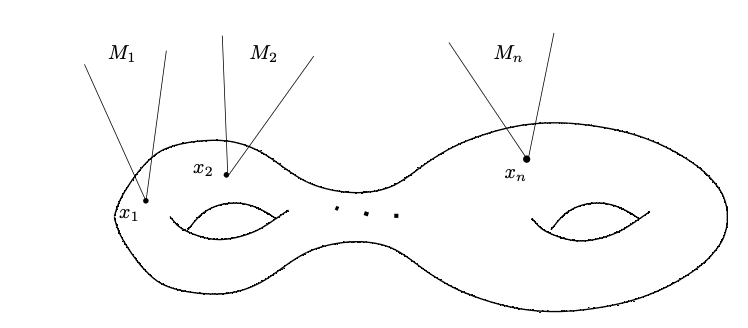
\includegraphics[width=0.6\textwidth]{Screenshot 2024-08-21 at 11.44.52 AM.png}
  %\caption{This is the caption of the image.}
  \label{fig:example_image}
\end{figure}
\end{frame}


\begin{frame}{Conformal Blocks}
We have an action of $\mathfrak{g}_{out} :=\mathfrak{g}[X\setminus \{x\}]$ on $V_k (\mathfrak{g})$ by taking residues. FBZ show that the space of conformal blocks can be identified as $\mathfrak{g}[X\setminus x]$ invariant functionals on $V_k (\mathfrak{g})$. 
\begin{block}{theorem}


$$ H_0 ( \mathfrak{g} \otimes R\Gamma(X, \mathcal{O}_X), \C) \simeq \operatorname{V}_{\mathfrak{g},k} / \mathfrak{g}[X \backslash x] \cdot \operatorname{V}_{\mathfrak{g},k} $$
\end{block}


\end{frame}


\begin{frame}{Raviolo Vertex Algebra}
    A raviolo vertex algebra is an  algebra with multiplication paramterized by the formal raviolo 
    \[
        \mathbb{R}\mathrm{av} = \mathbb{D} \cup_{\mathbb{D}^\times} \mathbb{D}.
    \]
    Distributions on the formal raviolo are given by 
    \[
    \mathcal{K}_{dist}:= \C[[z]] \oplus (\prod_{n\geq 0 } \C \Omega_z^{n}).
    \]
    formal raviolo Laurent series 
    \[
        \mathcal{K} := \C[[z]] \oplus (\oplus_{n\geq 0 } \C \Omega_z^n).
    \]
    A raviolo field on $V$ is an element $A(z) \in \mathrm{End}(V)\otimes \mathcal{K}_{dist}$ such that for any $B\in V$
    \[
    A(z)B \in V \otimes \mathcal{K}
    \]
\end{frame}

\begin{frame}{Raviolo Vertex Algebra}
    \begin{block}{Definition}
        A Raviolo Vertex Algebra is the data $(V, |0\rangle , \partial, Y) $ where

    \begin{itemize}
        \item $V = \oplus V^r$ is a $\Z$ graded vector space
        \item $|0\rangle  \in V^0$ is a distinguished element (vacuum vector).
        \item $ \partial : V \to V$ is an endomorphism of degree 0 (the translation operator).
        \item $Y= Y(-,z):V \to \mbox{End}(V) \otimes \mathcal{K}_{dist}$ is a linear map of degree 0.

    \end{itemize}

    The data is required to satisfy the following axioms ...
    \end{block}
\end{frame}

\begin{frame}{Raviolo Vertex Algebra}
    \begin{block}{Definition Continued}
        \begin{enumerate}
        \item For any $A \in V$ the element $Y(A,z)$ is a raviolo field.
        \item One has
              \[
                  [\partial,Y(A,z)] = \partial_z Y(A,z)
              \]
              for any $A \in V$ (translation axiom).
        \item The vacuum vector satisfies $\partial |0 \rangle = 0 $, $Y(|0\rangle,z) = Id$, and for any $A\in V$, $Y(A,z)|0\rangle \in V[[z]]$ and $Y(A,z=0)|0\rangle = A$ (vacuum axiom).
        \item For any $A,B\in V$ the fields $Y(A,z), Y(B,z)$ are mutually local.
    \end{enumerate}
    \end{block}
\end{frame}

\begin{frame}{Raviolo Current Vertex Algebra}
We can define the following Lie algebra $\mathfrak{g}\langle \langle u \rangle \rangle:= \mathfrak{g} \otimes \mathcal{K}$ with 1-shifted central extension 
   \[
         0 \to \C \kappa[-1] \to \hat{\mathfrak{g}}_{h} \to \mathfrak{g}\langle \langle u \rangle \rangle \to 0,
     \]
     \[
         [A \otimes \alpha, B \otimes \beta] := [A,B] \otimes \alpha \beta - \kappa h(A,B) \mbox{Res}_u du \alpha \partial_u \beta
     \]
     with residues defined as $\mbox{Res}_u dz u^n \Omega^{m}_z = \delta_{n,m}$.
     Let $\C_{\kappa} = \mbox{Sym}(\C\kappa[-1])$ be the representation of the Lie subalgebra $\C \kappa[-1] \oplus \mathfrak{g}[[u]]\subseteq \mathfrak{g}_h$ where $\kappa$ acts by multiplication by $\kappa$ and $\mathfrak{g}[[u]]$ .
     The induced $U(\hat{\mathfrak{g}}_h)$ module is a raviolo vertex algebra
     \[
         V[\mathfrak{g},h] : = U(\hat{\mathfrak{g}}_h) \otimes _{U(\hat{\mathfrak{g}}_{\geq 0})} \C_{\kappa}.
     \]
     The generating vertex operators are
     \[
         Y(\mu_{a,0}|0\rangle,z) = \sum_{n\geq 0 }z^n \mu_{a,n} + \Omega^n_{z} J_{a,n}
     \]
     for $\mu_{a,n}:= T_a \otimes \Omega^n_z$ and $J_{a,n}=T_a \otimes z^n$, for $(T_i)_{i=1}^n$ a basis of $\mathfrak{g}$
\end{frame}

\begin{frame}[fragile]{Translation Invariance}
    \begin{block}{Definition}
            For a manifold $M$ with a $G$ action, a prefactorization algebra, $\mathcal{F}$, is $G$-equivariant if for each $g \in G$ and each open $U\subseteq M$ we have isomorphisms
    \[
       \sigma_g: \mathcal{F}(U) \to \mathcal{F}(g \cdot U)
       \]
    which satisfy the following:
    \begin{itemize}
       \item For any $g,h \in G$ and $U \subseteq M$,
             \[
                \sigma_g \circ \sigma_h = \sigma_{gh} : \mathcal{F}(U) \to \mathcal{F}(ghU).
             \]
       \item For disjoint opens $U_1,\dots,U_k \subseteq V$, the following commutes
             \[
                \begin{tikzcd}
                   \mathcal{F}(U_1)\otimes \cdots \otimes \mathcal{F}(U_k) \ar[r,"\sigma_g"]  \ar[d]& \mathcal{F}(g U_1) \otimes \cdots \otimes \mathcal{F}(g U_k) \ar[d] \\
                   \mathcal{F}(V) \ar[r,"\sigma_g"] & \mathcal{F}(gV)
                \end{tikzcd}
             \]
             where the vertical arrows are the structure maps of the prefactorization algebra.
    \end{itemize}
    \end{block}
\end{frame}

\begin{frame}{Operad}
    The operad $B^3$ has operations given by configurations of balls. It is colored by the radius of the balls. Denote 
    \[
    B_3(r_1,\dots,r_k|s)
    \]
    as the configurations of balls of radius $r_i$ all disjoint and contained in $B^3_s(0)$. Composition is given by removing the intermediate ball.
    Translation invariant prefactorization algebras are algebras over this operad. Let $\mathcal{F}_r := \mathcal{F}(B^3_r(0))$. For each $p\in B_3(r_1,\dots,r_k|s)$ we have a map 
    \[
    m[p]:\mathcal{F}_{r_1}\times \dots \times \mathcal{F}_{r_k} \to \mathcal{F}_s
    \]
    If this is smooth, it is smoothly translation invariant.
\end{frame}


\begin{frame}{Cooperad}
    We can define a cooperad $C^\infty(B^3)$ which is defined by taking smooth functions on the operations on $B^3$ and using pull back $\circ_i^*$ of the composition map. A smoothly translation-invariant prefactorization algebra defines an algebra over this colored cooperad as we have a map
    \[
    \mu(r_1,\dots,r_k|s) \in C^\infty(B^3(r_1,\dots,r_k|s),\mathrm{Hom}(\mathcal{F}_{r_1},\dots ,\mathcal{F}_{r_k}|\mathcal{F}_s))
    \]
\end{frame}

\begin{frame}{Topological-Holomorphic (TH) Prefactorization Algebras}
    \begin{block}{Topological-Holomorphic Translation Invariant Prefactorization Algebra on $\C^n$}
        \begin{itemize}
            \item A prefactorization algebra on $\C\times \R$ where the natural action of the real Lie algebra $\mathbb{R} \times \C$ extends to the complexified Lie algebra $\R^{2n}\otimes \C$.
            \item Derivations $\eta,\xi$ of cohomological degree $-1$ such that 
            \[
            d\eta= \frac{\partial}{\partial \bar{z}}  \qquad d\xi = \frac{\partial}{\partial t}
            \]
            \[
            [\eta,\xi]=0
            \]
            \[
            [\eta,\frac{\partial}{\partial \bar{z}}] = 0 \qquad [\xi,\frac{\partial}{\partial t}]=0
            \]
        \end{itemize}
        where $d$ is the natural differential on the dg-Lie algebra $\mbox{Der}(\mathcal{F})$.
    \end{block}
\end{frame}

\begin{frame}{Dolbeaut-de Rham Cohomology}
The Dolbeaut-de Rham complex on $\C \times \R$ is denoted $\mathcal{A}^{0;*}(\C\times \R)$. $\mathcal{A}^{0;n}(\C\times \R)$ is the subspace of $n$-forms generated by $dt$ and $d\bar{z}$. The differential is $d'=\bar{\partial}+d_{dR}$.

We can define a cooperad $\mathcal{A}^{0;*}$ by taking Dolbeaut-de Rham forms on $B^3$
\end{frame}


\begin{frame}{Descent}
    \begin{block}{Theorem}
    Let $\mathcal{F}$ be a topological-holomorphic translation invariant prefactorization algebra on $\C\times \R$. Then $\mathcal{F}$  defines an algebra over the cooperad $\mathcal{A}^{0;*}(B^{3})$ valued in differentiable cochain complexes. This means that $m[p]$ lifts to a map
    \[
        \mu^{d'}(r_1,\dots,r_k|s):\mathcal{F}_{r_1} \times \dotsb \times \mathcal{F}_{r_k} \to \mathcal{A}^{0;*}(B_3(r_1,\dots,r_k|s), \mathcal{F}_s )
    \]
    compatible with the differentials. These maps also satisfy the following properties which make it an algebra over the cooperad $\mathcal{A}^{0;*}(B^3)$.
    \end{block}
    
\end{frame}



\begin{frame}{TH Pre-FA to Raviolo Vertex Algebra}
\begin{block}{Theorem}
Let $\mathcal{F}$ be a unital $U(1)$-equivariant topological-holomorphic translation invariant prefactorization algebra on
    $\C\times \R$ valued in differentiable vector spaces. Let $\mathcal{F}_k(B^3_r(0))$ be the weight $k$ eigenspace of the $U(1)$
    action on $\mathcal{F}(B^3_r(0))$. Assume the following
    % Assume that for each $B^3_r(0)$ the action of $U(1)$ on$\mathcal{F}(B^3_r(0))$ is tame.
    \begin{itemize}
        \item For, $r<r'$ the structure  map
              \[
                  \mathcal{F}_k(B^3_r(0)) \to \mathcal{F}_k(B_{r'}(0))
              \]
              is a quasi-isomorphism.
        \item For $k>>0$, the vector space $H^*(\mathcal{F}_k(B^3_r(0)))$ is zero.
        \item For each $k$ and $r$, we require that $H^*(\mathcal{F}_k(B^3_r(0)))$ is isomorphic, as a sheaf on the site of
              smooth manifolds, to a countable sequential colimit of finite dimensional graded vector spaces.
        \item The $U(1)$ action acts via rotations on $\C$.
    \end{itemize}
\end{block}
\end{frame}

\begin{frame}{Cohomological Laurent Expansion}
    \[
     H^{0;*}(\C\times \R \setminus\{\ubar{w}\}) = \begin{cases}
                \mathcal{O}_{hol}(\C)                        & *=0 \\
                \overline{\C[\partial_z] \omega(\ubar{z};0)} & *=1
            \end{cases}
    \]
    Denote $\Omega_z^n :=\frac{1}{n!}\partial_z^n \omega(\ubar{z},0)$ which is an analog of $z^{-n}$,
    \[
    \int_{S^2(0)}z^n dz \Omega^m_z = \delta_{n,m}.
    \]
    Define the cohomological Laurent expansion 
    \[
    \mathcal{L}' \alpha=\int_{S^2(0)}\sum_{i\geq 0} \Omega^i_z \tau^i \alpha+ \sum_{j\geq 0 } \lambda^j z^{j} dz \alpha
    \]
    Then identify $\tau^i$ with $z^i$ and $\lambda^i$ with $\Omega^i_z$.
\end{frame}

\begin{frame}{TH Pre-FA to Vertex Algebra}
    For $V= \oplus_{k \in \Z}  H^*(\mathcal{F}(B^3_r))$ we have an element
    \[
    m_{z,0}(-,-)\in H^{0;*}((\C \times \R)\setminus \{0\}, \mathrm{Hom}(V\otimes V,V)).
    \]
    A vertex operator is extracted by the expansion
    \[
    \mathcal{L}' m_{z,0}(A,B) \in V\langle \langle z \rangle \rangle
    \]
    \textcolor{red}{add diagram}
\end{frame}

\begin{frame}{Locality}
    The composition of vertex operators is given by 
    \[
    \mathcal{L}'_z \mathcal{L}'_w m_{z,w,0}(a,b,c)= Y(a,z)Y(b,w)c
    \]
    where we integrate $z$ over a larger sphere than $w$. Then the following cycle relation 
    \begin{tikzpicture}[every node/.style={font=\small}]

        % ==================================================
        % Left figure (big sphere + smaller sphere inside)
        % ==================================================
        \begin{scope}[xshift=0cm]  % Move this group to the left
          % -- Big sphere
          \shade[ball color=gray!30, opacity=0.4] (0,0) circle (1.2);
          %    Equator of the big sphere (flatten y by factor 0.3):
          %    top half: dashed
          \draw[dashed, opacity=0.3]
          plot[domain=0:180] ({1.2*cos(\x)},{0.3*1.2*sin(\x)});
          %    bottom half: solid
          \draw[opacity=0.3]
          plot[domain=180:360] ({1.2*cos(\x)},{0.3*1.2*sin(\x)});

          % -- Smaller sphere inside
          \shade[ball color=gray!30, opacity=0.7] (0,0) circle (0.8);
          %    Equator of the smaller sphere (radius=0.6, flatten y=0.15):
          \draw[dashed, opacity=0.5]
          plot[domain=0:180] ({0.8*cos(\x)},{0.8*0.25*sin(\x)});
          \draw[opacity=0.5]
          plot[domain=180:360] ({0.8*cos(\x)},{0.8*0.25*sin(\x)});

          % -- Black points & labels
          \fill[black] (0.83,0.83) circle (2pt)
          node[above] {$z$};
          \fill[black] (-0.4,0.4) circle (2pt)
          node[left] {$w$};


        \end{scope}

        % ==================================================
        % Middle figure (another big sphere + smaller sphere)
        % ==================================================
        \begin{scope}[xshift=4.0cm]  % Shift this figure to the right
          % -- Big sphere
          \shade[ball color=gray!30, opacity=0.4] (0,0) circle (0.8);
          %    Equator (flatten y by 0.25)
          \draw[dashed, opacity=0.5]
          plot[domain=0:180] ({0.8*cos(\x)},{0.25*0.8*sin(\x)});
          \draw[opacity=0.5]
          plot[domain=180:360] ({0.8*cos(\x)},{0.25*0.8*sin(\x)});

          % -- Smaller sphere
          \shade[ball color=gray!30, opacity=0.7] (0,0) circle (0.4);
          %    Equator for smaller sphere (radius=0.4, flatten=0.125):
          \draw[dashed, opacity=0.7]
          plot[domain=0:180] ({0.4*cos(\x)},{0.4*0.125*sin(\x)});
          \draw[opacity=0.7]
          plot[domain=180:360] ({0.4*cos(\x)},{0.4*0.125*sin(\x)});

          % -- Black points & labels
          \fill[black] (-0.3,0.3) circle (2pt)
          node[left] {$z$};
          \fill[black] (0, 0.8) circle (2pt)
          node[above] {$w$};
        \end{scope}

        % ==================================================
        % Right figure ("snowman": two stacked spheres)
        % ==================================================
        \begin{scope}[xshift=8.0cm]
          % -- Lower sphere
          \shade[ball color=gray!30, opacity=0.4] (0,0) circle (0.8);
          %    Equator, flatten=0.25
          \draw[dashed, opacity=0.5]
          plot[domain=0:180] ({0.8*cos(\x)},{0.25*0.8*sin(\x)});
          \draw[opacity=0.5]
          plot[domain=180:360] ({0.8*cos(\x)},{0.25*0.8*sin(\x)});

          % -- Upper sphere
          %    Center at (0,1.0), radius=0.5
          \shade[ball color=gray!30, opacity=0.7] (0,0.8) circle (0.4);
          %    Equator for the top sphere (flatten=0.2)
          \draw[dashed, opacity=0.7]
          plot[domain=0:180] ({0.4*cos(\x)},{0.8 + 0.4*0.14*sin(\x)});
          \draw[opacity=0.7]
          plot[domain=180:360] ({0.4*cos(\x)},{0.8 + 0.4*0.14*sin(\x)});

          % -- Black points & labels

          \fill[black] (0, 0.8) circle (2pt)
          node[above] {$w$};
          \fill[black] (0.35, 0.9) circle (2pt)
          node[right] {$z$};

        \end{scope}

      \end{tikzpicture}
      The commutator is given by the integral over the third cycle. 
\end{frame}

\begin{frame}{Locality}
    It can be shown that 
    \[
    m_{\ubar{w},0}(m_{\ubar{w},\ubar{z}}(b,a),c) = c(z,w) + \sum_{i=0}^N \Omega_{z-w}^i C_i(w).
    \]
    Then by direct computation one can check that 
    \[
    [\mathcal{L}'_z,\mathcal{L}'_w]\Omega^{n}_{z-w} C_n(w) = \Delta^{(n)}(z-w) C_n(w)
    \]
    and 
    \[
    [\mathcal{L}'_z,\mathcal{L}'_w] c(z,w) = 0.
    \]
    This shows that the fields constructed from the prefactorization algebra are mutually local.
\end{frame}

\begin{frame}{Raviolo Current Factorization Algebra}
    For $\mathfrak{g}$ a Lie algebra, $M$ a manfiold with THF and $\kappa: \mathfrak{g}^{\otimes 2} \to \C$ a $\mathfrak{g}$ invariant symmetric pairing define the precosheaf of dg-Lie algebras
    \[
    \mathcal{G}^{M} :U \to (\mathcal{A}^{0;*}_c(U)\otimes \frak{g}, d')
    \]
    Then define the 2-shifted central extension for $f(t)\otimes X, g(t)\otimes Y$ by
    \[
    -\left( \int_U f \partial g \right) \kappa(X,Y) c
    \]
    The raviolo current factorization algebra is the factorization envelope of $\hat{\mathcal{G}}^\Sigma :=\mathcal{G}^\Sigma \oplus c\C[-2]$, or, 
    \[
    \mathcal{F} := C_*(\hat{\mathfrak{g}}^\Sigma )
    \]
    with the Chevalley-Eilenberg differential.
    \begin{block}{Theorem (CG)}
        The raviolo vertex algebra defined by $\mathcal{F}$ on $\C\times \R$ is the raviolo current vertex algebra.
    \end{block}
\end{frame}


\end{document}